\chapter{Tecnica Ottimizzata}

In questo capitolo viene presentata un'ottimizzazione al problema descritto nel capitolo precedente.
Tale ottimizzazione si basa sul principio delle decomposizioni bilanciate.
Si fa vedere, inoltre, come l'utilizzo di quest'ultima permetta un notevole miglioramento delle performance.

\section{Decomposizioni Bilanciate di un albero}
Si vuole andare a dimostrare in questa sezione, che dato un albero T \`e sempre possibile ricavare una scomposizione bilanciata dell'albero.
\\
Prima di poter enunciare e dimostrare il risultato principale di questa sezione occorre dare delle nozioni preliminari.

\newtheorem{definizione}{Definizione}[section]

\begin{definizione}
	\label{definizioneDeco}
Sia $T_r$ un albero radicato nel nodo r, con k nodi.
Diremo che la coppia (A,B), dove  A e B sono insiemi contenenti i nodi di $T_r$, \`e una decomposizione per l'albero $ T_r $ se:
\begin{itemize}
	\item $| A | + | B | = k$
	\item $A \cap B = \{r\}$.
\end{itemize}
\end{definizione}


\begin{definizione}
\label{lemmaDeco}
Dato un albero $ T $, diremo che $ (A,B) $ \`e una decomposizione bilanciata se:
\begin{equation*}
	\max{ \{|A| , |B| \} }  \le  f(k)
\end{equation*}
\end{definizione}





\begin{definizione}
Per ogni nodo $ v $ di un albero $ T $, le diramazioni di $ T $  rispetto a $ v $, sono tutti i sottoalberi massimali, radicati nei figli di $ v $. 
Sia  $\alpha(v)$  , $ \forall v \in T $,il grado della diramazione di $ v $ con il maggior numero di nodi.

Un nodo $ v $ di un albero $ T $ con $ n $ nodi, \`e un nodo centroide se $\alpha(v)\le\frac{n}{2}$.
\end{definizione}\mbox{}

Il centroide di un albero non \`e necessariamente unico, infatti Jordan \cite{jordan1869assemblages}  ha dimostrato che o (i) $ T $ ha un singolo centroide $ v $ e $\alpha(v) < \frac{n}{2}$ oppure (ii) $ T $ ha due nodi centroidi (adiacenti) $v_1$ e $v_2$ tali che $\alpha(v_1) = \alpha(v_2) = \frac{n}{2}$, in questo caso il numero di nodi $ n $ \`e pari.\\
Esistono diversi algoritmi per la ricerca del centroide, quello utilizzato in questa tesi \`e l'algoritmo di Jordan \cite{jordan1869assemblages} che  ha una complessit\`a temporale lineare nel numero di nodi. \\
Il primo passo da effettuare \`e determinare $\alpha(v)$ per ogni nodo $ v \in T$.\\
Viene definito $ \alpha(v) = \max\{\delta(z_i)\} $, dove $ \delta(z_i )$ rappresenta il grado di diramazione, ossia il numero di nodi incontrati durante una visita DFS (in profondit\`a) effettuata a partire da ogni nodo radice, $ z_i $, di tutte le possibili diramazioni di $ v $.
Una volta calcolato il valore di $ \alpha(v) $, $ \forall v \in T $, si verifica per quali valori di $ \alpha(v) $ risulta $\alpha(v)\le\frac{n}{2}$.
Nel caso ci fosse un unico nodo $ v $, come in (i), che soddisfa la precedente espressione, allora tale nodo rappresenta l'unico  centroide dell'albero $ T $.
Nel caso, invece, ce ne fossero due, come definito in (ii), per esempio $ v_1 $ e $ v_2 $,  l'albero $ T $ conterr\`a due centroidi, rispettivamente $ v_1 $ e $ v_2 $.\\
Nell'esempio \ref{es1} si pu\`o vedere l'applicazione dell'algoritmo per la ricerca del centroide.
	\begin{figure}[htbp]
		\centering
		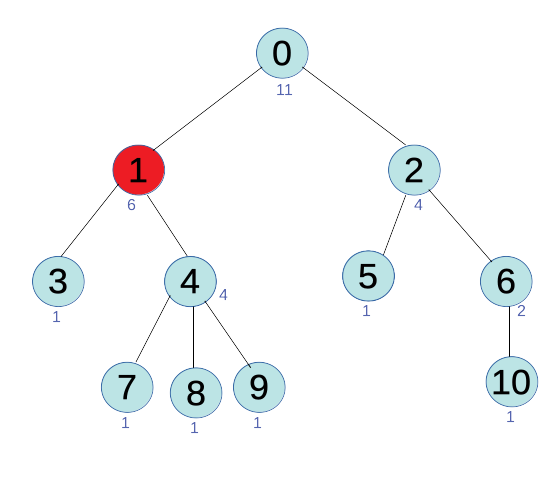
\includegraphics[width=5cm]{capitolo3/grafo2}
		\caption{Albero $ T $  per la ricerca del centroide} 
		\label{fig:2}
\end{figure}
\mbox{}\\

\newtheorem{esempio}[definizione]{Esempio}
\begin{esempio}
	\label{es1}
Si consideri l'albero T in figura \ref{fig:2} per la ricerca del nodo centroide.
Su tutti i di $ T $, numerato da 0 a 10,  viene calcolato $\alpha(v)$ . \\
Quello che si ottiene \`e :

%$\alpha(0) = 6$; $\alpha(1) = 5$; $\alpha(2) = 7$; $\alpha(3) = 10$; $\alpha(4) = 7$; $\alpha(5) =  10$ $\alpha(6) = 9$; $\alpha(7) = 10$; $\alpha(8) = 10$; $\alpha(9) = 10$; $\alpha(10) = 10$.


\begin{center}
	\begin{tabular}{ c c c c c  }
		$\alpha(0) = 6$ & & $\alpha(1) = 7$ & & $\alpha(2) = 5$ \\ 
		$\alpha(3) = 9$ && $\alpha(4) = 10$ &&  $\alpha(5) =  7$ \\  
		$\alpha(6) = 10$ && $\alpha(7) = 10$ && $\alpha(8) = 10$ \\
		$\alpha(9) = 10$ && $\alpha(10) = 10$ &&
	\end{tabular}
\end{center}

Poich\'e $ \left\lfloor\frac{n}{2} \right\rfloor = \left\lfloor \frac{11}{2} \right\rfloor = 5$, l'unico nodo per cui la disuguaglianza risulta vera \`e il nodo 2, infatti $5\le 5$, ed \`e esattamente l'unico centroide dell'albero T (figura \ref{fig:2}). 
\demo
\end{esempio}\mbox{}\\

L'ultimo punto da considerare prima di poter enunciare e dimostrare il risultato principale di questa sezione riguarda la definizione di un algoritmo valido per comporre due insiemi di nodi $ A $ e $ B $,in modo bilanciato.
Siano dati in input un albero $ T $,con $ k $ nodi, ed un fattore di bilanciamento definito da una funzione $ f(k) $.
Inizialmente viene posta la radice $ r $ di $ T $ come unico nodo nei due insiemi $ A $ e $ B $.
Successivamente, si verifica se la cardinalit\`a del sottoalbero radicato nel figlio pi\`u a sinistra di $ r $ sommata alla cardinalit\`a corrente dell'insieme $ A $ non supera il valore della funzione $ f(k) $.
In caso affermativo si aggiungono tutti i nodi del sottoalbero radicato nel figlio pi\`u a sinistra di $ r $ nell'insieme $ A $ e si ripete il passo descritto in precedenza sul sottoalbero radicato nel figlio successivo di $ r $.
Quando, al generico passo $ i $, la cardinalit\`a dell'insieme $ A $, fino a quell'istante, sommata alla cardinalit\`a del sottoalbero radicato nell'$ i$-esimo figlio di $ r $ supera il valore della funzione $ f(k) $, i nodi dell'$ i$-esimo sottoalbero e di tutti quelli a seguire verranno aggiunti nell'insieme $ B $.
Poich\`e i nodi dell'albero sono in numero finito \`e garantito che l'algoritmo si arresta in un tempo finito.\\


In base a tutte le nozioni illustrate in precedenza possiamo passare ad enunciare il seguente teorema.


\newtheorem{teorema1}[definizione]{Teorema}
\begin{teorema1}
Per ogni albero T di k nodi esiste un nodo r di T , tale che l'albero $T_r$, ottenuto radicando T in r ammette una decomposizione $ \lceil \frac{2}{3}k \rceil$-bilanciata.
\end{teorema1}
\begin{proof}
	Sia $ T $ un albero con pi\`u di due nodi (per $n\le2$ la propriet\`a \`e banalmente vera). \\
	La prima operazione da compiere \`e individuare il nodo $ r $ di $ T $, su cui si andr\`a poi a radicare il nuovo albero $ T_r $.\\
	Per come \`e stato definito, il nodo da ricercare, non \`e altro che  un centroide dell'albero $ T $, quindi si applica l'algoritmo precedentemente descritto per la sua ricerca.\\ 
	Una volta trovato si eseguono opportune modifiche su $ T $ in modo da radicarlo nel suo centroide, ottendendo cos\`i $ T_r $.\\ 
	Senza perdere di generalit\`a, si suppone che i sottoalberi radicati nei figli di r siano ordinati in maniera non crescente rispetto alla loro dimensione.\\
	\`E possibile ottenere una scomposizione, (A,B), dei k nodi di $T_r$,  tale che, applicando l'algoritmo descritto in precedenza con fattore di bilanciamento $ f(k) = \left\lceil \frac{2}{3} \right\rceil $, gli insiemi $ A $ e $ B $ risultino bilanciati.
	Risulta, pertanto, che l'insieme con il maggior numero di elementi non contiene pi\`u dei $\left\lceil \frac{2}{3} \right\rceil$ del totale dei nodi. \\
	Sia esso, ad esempio, l'insieme $ A $.
	Si denota con $ x $ il primo sottoalbero di $ T_r $ non appartenente ad $  A $, radicato nell'$ i $-esimo figlio della radice di $ T_r $ (figura \ref{fig:4}).
	\begin{figure}[htbp]
		\centering
		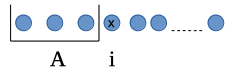
\includegraphics[width=6cm]{capitolo3/3}
		\caption{}
		\label{fig:4}
	\end{figure}
	
	Si possono verificare  due casi:
	\begin{itemize}
		\item (i=2)  L'insieme A \`e formato dall'insieme di nodi di un unico sottoalbero y:
		\begin{figure*}[htbp]
			\centering
			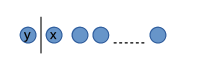
\includegraphics[width=6cm]{capitolo3/4}
			\caption{}
		\end{figure*}\\
		Per costruzione di $ A $, si ha che:
		\\
		\begin{equation}
			\label{dis1}
			|y| + |x| > \frac{2}{3}k
		\end{equation}
		\\
		Dividendo entrambi i membri di (2) per  due, si ottiene:
		\\
		\begin{equation}
			\frac{ |x| + |y| }{2} > \frac{k}{3}  
		\end{equation}
		\\
		Si pu\`o notare che $\frac{ |x| + |y| }{2} $ rappresenta esattamente il valore medio. \\
		Dall'ordinamento dei sottoalberi di $T_r$, risulta che il sottoalbero indicato con $ y $ \`e maggiore o uguale a quello indicato con $ x $.\\
		Pertanto :
		\\
		\begin{equation}
			y \ge \frac{ x + y }{2} 
		\end{equation}
		\\
		Combinando le disequazioni (2) e (3) si ottiene:
		\\
		\begin{equation*}
			y > \frac{k}{3}  
		\end{equation*}
		\\
		\item ($i\ge3$) In $ A $ ci sono almeno due elementi. Sia $ S $ la cardinalit\'a dell'insieme $ A $.
		
		\begin{figure*}[htbp]
			\centering
			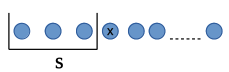
\includegraphics[width=6cm]{capitolo3/5}
			\caption{}
		\end{figure*}
	
		Sommando $ S $ alla cardinalit\`a di $ x $ si ha:
		\\
		\begin{equation}
			S + |x| > \frac{2}{3}
		\end{equation}
		\\
		Inoltre, avendo un ordinamento ben definito dei sottoalberi di $ T_r $, ne consegue che:
		\\ 
		\begin{equation}
			|x| \le \frac{k}{3}
		\end{equation}
		\\
		Sottraendo la diseguazione (6) alla disequazione (5), si ottiene:
		\\
		\begin{equation}
			S + |x| - |x| > \frac{2}{3} k - \frac{k}{3} \hspace{0.3cm} \text{    ossia    }\hspace{0.3cm} S > \frac{k}{3}
		\end{equation}
		\\
		Perci\`o gli insiemi ottenuti dalla scomposizione di $T_r$ hanno cardinalit\`a compresa tra $\frac{1}{3} k$ e $\frac{2}{3} k$, garantendo cos\`i delle decomposizioni bilanciate.
	\end{itemize}
\end{proof}\mbox{}\\

	Nel caso in cui si abbiano due centroidi, la scelta su quale radicare l'albero  \`e deterministica e  viene fatta prendendo quello che, tra i due, garantisce un'ordinamento corretto dei sottoalberi radicati nella radice oppure, a parit\`a di ordinamento, ne viene scelto uno dei due in maniera arbitraria. 


